% ============================================================
%  Příprava na maturitu – Elektrotechnika
%  Okruh 12: Polovodičové součástky
% ============================================================

\documentclass[a4paper,10pt]{article}

\usepackage[T1]{fontenc}
\usepackage[utf8]{inputenc}
\usepackage[left=2.0cm, right=1.8cm, top=1.8cm, bottom=1.8cm]{geometry}
\usepackage{parskip}
\usepackage{xcolor}
\usepackage{tabularx}
\usepackage{booktabs}
\usepackage{tikz}
\usepackage{mdframed}
\usepackage{amsmath}
\usepackage{enumitem}
\usepackage{circuitikz}

\usetikzlibrary{arrows.meta, positioning, decorations.pathmorphing, shapes.geometric, calc}

% --- Barvy ---
\definecolor{accent}{HTML}{1A3A5C}
\definecolor{lightblue}{HTML}{EAF2F8}
\definecolor{lightyellow}{HTML}{FDFBE4}
\definecolor{lightgreen}{HTML}{EAF7EA}
\definecolor{lightred}{HTML}{FDE8E8}
\definecolor{lightgray}{HTML}{F4F4F4}

% --- Boxy ---
\newmdenv[backgroundcolor=lightblue,linecolor=accent!40,roundcorner=4pt,
  innertopmargin=6pt,innerbottommargin=6pt,innerleftmargin=8pt,innerrightmargin=8pt]{pojmybox}
\newmdenv[backgroundcolor=lightyellow,linecolor=accent!30,roundcorner=4pt,
  innertopmargin=6pt,innerbottommargin=6pt,innerleftmargin=8pt,innerrightmargin=8pt]{vysvetlenibox}
\newmdenv[backgroundcolor=lightgreen,linecolor=accent!40,roundcorner=4pt,
  innertopmargin=6pt,innerbottommargin=6pt,innerleftmargin=8pt,innerrightmargin=8pt]{vzorcebox}
\newmdenv[backgroundcolor=lightred,linecolor=accent!30,roundcorner=4pt,
  innertopmargin=6pt,innerbottommargin=6pt,innerleftmargin=8pt,innerrightmargin=8pt]{durazbox}

\setlist[itemize]{noitemsep, leftmargin=1.4em, topsep=2pt}
\setlist[enumerate]{noitemsep, leftmargin=1.4em, topsep=2pt}

% --- Zkratka pro jednotky ---
\newcommand{\jednotka}[1]{\,[\mathrm{#1}]}

\begin{document}

% ============================================================
\section*{\large Okruh 12 – Polovodičové součástky}

\begin{pojmybox}
\textbf{Klíčové pojmy:}
polovodič (křemík), typ P a N, PN přechod, propustný a závěrný směr, usměrňovací dioda, Zenerova dioda, LED, bipolární tranzistor (NPN/PNP), unipolární tranzistor (MOSFET), tyristor, VA charakteristika
\end{pojmybox}

\begin{vysvetlenibox}

% ================================================================
\subsection*{1. Princip polovodičů a PN přechod}

Polovodiče (nejčastěji křemík Si) mají elektrickou vodivost mezi vodiči a izolanty. Jejich vodivost lze radikálně změnit dodáním tepla, světla nebo **příměsí** (dotováním).

\textbf{Příměsové polovodiče:}
\begin{itemize}
    \item \textbf{Typ N (Negativní):} Přidáním pětivazného prvku (fosfor) získáme **nadbytek volných elektronů**.
    \item \textbf{Typ P (Pozitivní):} Přidáním trojvazného prvku (bór) získáme nedostatek elektronů, vznikají tzv. **díry** (chovají se jako kladný náboj).
\end{itemize}

\textbf{PN Přechod (Základ diody):} Spojením typu P a N vznikne na rozhraní oblast bez volných nábojů (hradlová vrstva).
\begin{itemize}
    \item \textbf{Propustný směr:} Kladný pól zdroje na P (Anoda), záporný na N (Katoda). Vrstva se zúží a **proud prochází**.
    \item \textbf{Závěrný směr:} Kladný pól na N, záporný na P. Hradlová vrstva se rozšíří a **proud neprochází**.
\end{itemize}

% ================================================================
\subsection*{2. Diody a jejich vlastnosti}

Dioda je dvoupólová součástka využívající jeden PN přechod. Propouští proud jen jedním směrem.

\begin{center}
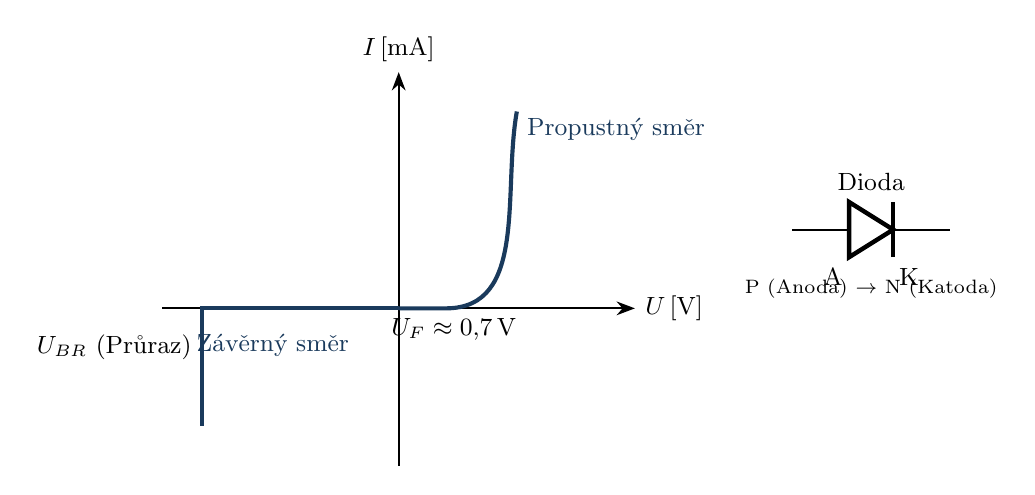
\begin{tikzpicture}[>=Stealth, font=\small, thick]
  % VA Charakteristika
  \draw[->] (-3,0) -- (3,0) node[right] {$U\,\mathrm{[V]}$};
  \draw[->] (0,-2) -- (0,3) node[above] {$I\,\mathrm{[mA]}$};
  
  % Křivka
  \draw[accent, line width=1.5pt] (0,0) -- (0.6,0) to[out=0, in=260] (1.5, 2.5);
  \draw[accent, line width=1.5pt] (0,0) -- (-2.5, 0) -- (-2.5, -1.5);
  
  % Popisky os
  \node[below] at (0.7,0) {$U_F \approx 0{,}7\,\mathrm{V}$};
  \node[above right, accent] at (1.5, 2) {Propustný směr};
  \node[below left, accent] at (-0.5, -0.2) {Závěrný směr};
  \node[left] at (-2.5, -0.5) {$U_{BR}$ (Průraz)};
  
  % Schematická značka
  \begin{scope}[xshift=5cm, yshift=1cm]
    \draw (0,0) to[D, l=Dioda, a=A \hspace{0.5cm} K] (2,0);
    \node[below, font=\scriptsize] at (1,-0.5) {P (Anoda) $\rightarrow$ N (Katoda)};
  \end{scope}
\end{tikzpicture}
\end{center}

\textbf{Speciální typy diod:}
\begin{itemize}
    \item \textbf{Usměrňovací dioda:} Přeměňuje střídavý proud na stejnosměrný.
    \item \textbf{Zenerova dioda:} Využívá se v **závěrném směru**. Při určitém napětí (Zenerovo napětí) se "prorazí" bez zničení a udržuje na sobě konstantní napětí. Slouží ke **stabilizaci napětí**.
    \item \textbf{LED (Svítivá dioda):} V propustném směru vyzařuje fotony. Úbytek napětí závisí na barvě ($U_F = 2\,\mathrm{V}$ pro červenou, $3\,\mathrm{V}$ pro bílou/modrou).
    \item \textbf{Fotodioda:} V závěrném směru reaguje na světlo (zvětšuje se závěrný proud).
\end{itemize}

\begin{center}
\begin{circuitikz}[font=\small, thick]
  \draw (0,0) to[zD, l=Zenerova d.] (2,0);
  \draw (3,0) to[leD, l=LED] (5,0);
  \draw (6,0) to[pD, l=Fotodioda] (8,0);
\end{circuitikz}
\end{center}

% ================================================================
\subsection*{3. Bipolární tranzistor (BJT)}

Obsahuje dva PN přechody (struktura **NPN** nebo **PNP**). Má tři vývody: \textbf{Báze (B), Kolektor (C), Emitor (E)}.
Slovo "bipolární" znamená, že se vedení proudu účastní oba typy nábojů (elektrony i díry).

\textbf{Princip (Typ NPN):} Mezi Kolektorem a Emitorem je velké napětí, ale obvod je zavřený. Pokud do Báze pustíme **malý proud** ($I_B$), tranzistor se otevře a mezi Kolektorem a Emitorem začne protékat **velký proud** ($I_C$).
Tranzistor funguje jako **proudový zesilovač** nebo **elektronický spínač**.

\begin{vzorcebox}
\[
I_C = \beta \cdot I_B \qquad \text{(v lineárním režimu)}
\]
kde $\beta$ (nebo $h_{FE}$) je proudový zesilovací činitel (běžně 100 až 500).
\end{vzorcebox}

\begin{center}
\begin{circuitikz}[font=\small, thick]
  % NPN
  \draw (0,0) node[npn] (npn) {};
  \node[left] at (npn.B) {B};
  \node[above] at (npn.C) {C};
  \node[below] at (npn.E) {E};
  \node[above=0.2cm, right=0.2cm, text=accent] at (npn.center) {\textbf{NPN}};
  \draw[->, red] (-1,0) -- (-0.5,0) node[midway, above] {$I_B$};
  \draw[->, blue] (0,1) -- (0,0.5) node[midway, right] {$I_C$};

  % PNP
  \begin{scope}[xshift=4cm]
    \draw (0,0) node[pnp] (pnp) {};
    \node[left] at (pnp.B) {B};
    \node[above] at (pnp.C) {C};
    \node[below] at (pnp.E) {E};
    \node[above=0.2cm, right=0.2cm, text=accent] at (pnp.center) {\textbf{PNP}};
  \end{scope}
  
  \begin{scope}[xshift=7cm, yshift=-1cm]
    \node[align=left, text width=6cm, font=\scriptsize, draw, fill=lightyellow, rounded corners=2pt, inner sep=4pt] at (0,1) {
      \textbf{Pomůcka k šipkám:}\\
      Šipka je vždy na Emitoru a ukazuje směr technického proudu (od P k N).\\
      \textbf{NPN:} Šipka ven.\\
      \textbf{PNP:} Šipka dovnitř (Půjdem Na Pivo).
    };
  \end{scope}
\end{circuitikz}
\end{center}

% ================================================================
\subsection*{4. Unipolární tranzistory (FET / MOSFET)}

Na rozdíl od bipolárních jsou řízeny \textbf{elektrickým polem (napětím)}, nikoliv proudem! Proud protéká pouze jedním typem materiálu (proto "unipolární"). Nejrozšířenější je **MOSFET** (Metal-Oxide-Semiconductor).

Má vývody: \textbf{Gate (G - Hradlo), Drain (D - Odtok), Source (S - Pramen)}.

\textbf{Princip:} Mezi hradlem (G) a zbytkem tranzistoru je tenká vrstvička izolantu (oxid křemičitý $\mathrm{SiO_2}$). Přiložením **napětí** na hradlo se elektrostatickou indukcí vytvoří vodivý kanál mezi D a S a tranzistor se otevře.

\begin{durazbox}
\textbf{Hlavní výhoda MOSFETu:}
Do hradla neteče prakticky **žádný proud** (odpor hradla jsou gigaohmy). Lze jím spínat obrovské výkony s téměř nulovou spotřebou řídicího obvodu. Tvoří základ všech dnešních procesorů a pamětí.
\end{durazbox}

\begin{center}
\begin{circuitikz}[font=\small, thick]
  \draw (0,0) node[nmos] (nmos) {};
  \node[left] at (nmos.G) {G};
  \node[above] at (nmos.D) {D};
  \node[below] at (nmos.S) {S};
  \node[right=0.2cm, text=accent] at (nmos.center) {\textbf{N-kanál}};
  \draw[<->, red] (-1,-0.8) -- (0, -0.8) node[midway, below] {$U_{GS}$ (řídicí napětí)};
  \draw[dashed] (-1, -0.8) -- (-1, 0) -- (nmos.G);
\end{circuitikz}
\end{center}

% ================================================================
\subsection*{5. Spínací součástky: Tyristor a Triak}

Bipolární tranzistory sice fungují jako spínače, ale pro velmi vysoké proudy a síťová napětí (AC) se využívá 4-vrstvá struktura (PNPN).

\begin{itemize}
    \item \textbf{Tyristor:} Má Anodu, Katodu a řídicí elektrodu (Gate). Propustí proud jen jedním směrem a to až poté, co dostane **krátký proudový impulz do Gate**. Zůstane otevřený, dokud proud mezi A a K neklesne k nule (skvělé pro fázové řízení výkonu).
    \item \textbf{Triak:} Jsou to v podstatě "dva tyristory zapojené antiparalelně". Propouští a spíná proud **oběma směry** (AC). Ideální pro stmívače osvětlení nebo regulaci otáček střídavých motorů (vysavače, vrtačky).
\end{itemize}

\begin{center}
\begin{circuitikz}[font=\small, thick]
  \draw (0,0) to[Ty, l=Tyristor, n=tyr] (2,0);
  \node[above] at (tyr.G) {G};
  \draw (4,0) to[Tr, l=Triak, n=tri] (6,0);
  \node[above] at (tri.G) {G};
\end{circuitikz}
\end{center}

% ================================================================
\subsection*{6. Shrnutí – BJT vs MOSFET}

\begin{center}
\begin{tabularx}{0.97\linewidth}{@{} l X X @{}}
\toprule
\textbf{Parametr} & \textbf{Bipolární (BJT)} & \textbf{Unipolární (MOSFET)} \\
\midrule
Řízeno & Proudem ($I_B$) & Napětím ($U_{GS}$) \\
Vývody & Báze, Kolektor, Emitor & Gate, Drain, Source \\
Vstupní odpor & Nízký (kiloohmy) & Obrovský (gigaohmy) \\
Rychlost spínání & Střední & Velmi rychlé \\
Použití v logických IO & Zastaralé (TTL) & Dominantní (CMOS, CPU) \\
\bottomrule
\end{tabularx}
\end{center}

\end{vysvetlenibox}

\end{document}
